\documentclass[12pt, a4paper]{article}

\usepackage[T1]{fontenc}
\usepackage{courier}

\usepackage[left=3cm, right=3cm, top=4cm, bottom=4cm]{geometry}
\usepackage{amssymb}
\usepackage{amsmath}
\usepackage{booktabs}
\usepackage{setspace}
\usepackage{float}
\usepackage{mathtools}
\usepackage{graphicx}
\usepackage[usenames,dvipsnames]{xcolor}
\usepackage{hyperref}
\usepackage{graphicx}
\graphicspath{./}
\usepackage{algorithm2e}
\usepackage{bm}

\newcommand{\code}[1]{\texttt{#1}}

\newcommand{\R}{\mathbb{R}}
\newcommand{\nulldelimiter}{.\kern-\nulldelimiterspace}
\newcommand{\divs}[2]{\left\nulldelimiter#1\middle|\right\nulldelimiter#2}
\newcommand{\bigO}{\mathcal{O}}

\DeclarePairedDelimiter{\floor}{\lfloor}{\rfloor}
\DeclarePairedDelimiter{\abs}{\lvert}{\rvert}

\title{
  Obliczenia Naukowe\\
  \begin{center}\Large Lista 5\end{center}
}
\author{Piotr Kocia}

\begin{document}

\maketitle
\tableofcontents

\section{Introduction}
The purpose of this document is to present a viable solution to the problem of
computing with large matrices of a particular structure. We are to solve a
simple system of equations
$$
\bm{Mx} = \bm{b}
$$
where $\bm{M} \in \R^{n \times n}$ and $\bm{b} \in \R^n$, $n \ge 4$ are known.
The matrix $\bm{M}$ is a band matrix and has the following structure
\begin{equation}
  \bm{M} =
  \begin{bmatrix}
    \bm{A}_1 & \bm{C}_1 & \bm{0} & \bm{0} & \bm{0} & \dotsi & \bm{0} \\
    \bm{B}_2 & \bm{A}_2 & \bm{C}_2 & \bm{0} & \bm{0} & \dotsi & \bm{0} \\
    \bm{0} & \bm{B}_3 & \bm{A}_3 & \bm{C}_3 & \bm{0} & \dotsi & \bm{0} \\
    \vdots & \ddots & \ddots & \ddots & \ddots & \ddots & \vdots \\
    \bm{0} & \dotsi & \bm{0} & \bm{B}_{v-2} & \bm{A}_{v-2} & \bm{C}_{v-2} & \bm{0} \\
    \bm{0} & \dotsi & \bm{0} & \bm{0} & \bm{B}_{v-1} & \bm{A}_{v-1} & \bm{C}_{v-1} \\
    \bm{0} & \dotsi & \bm{0} & \bm{0} & \bm{0} & \bm{B}_{v} & \bm{A}_{v}
  \end{bmatrix}
\end{equation}
$v = n / l$ with an imposed requirement $\divs{l}{n}$, where $l$ is the size of
the square matrices $\bm{A}_k, \bm{B}_k, \bm{C}_k \in \R^{l \times l}$.
$\bm{A}_k$ are dense matrices, while $\bm{B}_k, \bm{C}_k$ are defined to be as
follows
\begin{equation}
  \bm{B}_k =
  \begin{bmatrix}
    0 & \dotsi & 0 & b^k_1 \\
    0 & \dotsi & 0 & b^k_2 \\
    \vdots & & \vdots & \vdots \\
    0 & \dotsi & 0 & b^k_l
  \end{bmatrix}
\end{equation}
\begin{equation}
  \bm{C}_k =
  \begin{bmatrix}
    c^k_1 & 0 & 0 & \dotsi & 0 \\
    0 & c^k_2 & 0 & \dotsi & 0 \\
    \vdots & \ddots & \ddots & \ddots & \vdots \\
    0 & \dotsi & 0 & c^k_{l-1} & 0 \\
    0 & \dotsi & 0 & 0 & c^k_{l}
  \end{bmatrix}
\end{equation}

The difficulty stems from the size of the inputs. We are considering matrices up
to a million in size. The problem becomes intractable at those sizes due to
physical limitations of computers. At 8 bytes per entry, a naive representation
of the matrix $\bm{M}$ would require an astonishing 7450GiB of RAM, which enters
mainframe levels of RAM storage. Additionally, at $\bigO(n^3)$ time complexity,
assuming that each operation takes only one CPU cycle on a 1GHz CPU, Gauss
elimination would require 10779 days. It is thus clear that a more efficient
representation is required.

\section{The matrix structure}
The matrix $\bm{M}$ is sparse. Its density is less than $\frac{3v}{v^2} =
\frac{3}{v} = \frac{3l}{n}$. Since $l$ tends to be several orders of magnitude
smaller than $n$, the density is mostly significantly less than 0.1\%. Analysis
of the workings of the Gauss elimination and LU decomposition bring us to the
conclusion that the majority of the entries in the matrix $\bm{M}$ are always 0.
This observation drives us to use a structure that eliminates those entries.
Several such structures exist, commonly referred to as "sparse matrix", however,
the primary disadvantage of those is non-constant time access to the elements of
the matrix. We thus devise our own structure satisfying our requirements.

The idea is that we represent only the potentially non-zero part of each row. In
our applications, this happens to be a contiguous section spanning $\bm{B},
\bm{A}, \bm{C}$ and an overrun of length $l$ for a total of $4l$ contiguous
entries. We lay out the sections as a $n \times 4l$ matrix. Accessing a row is
trivial and is done in constant time by a simple indexing operation. Column
access is also a constant time indexing operation, however, it requires we map
the column from $\bm{M}$ to our representation. Each block of $l$ rows is offset
by $0l, 1l, 2l, ..., (v-1)l$, hence to read a value from our representation we
subtract the offset from the column index. If the resulting index falls in ${0,
..., 4l - 1}$, we return the corresponding value, otherwise the (non-existent)
entry would be a zero and we return 0. The offset is $\floor{\frac{r}{l}}l$,
where $r$ is the row index (assuming 0-based indexing).

The overrun section is only necessary because of the Gauss elimination with
partial selection of the primary element - the row swaps we perform there may
happen within blocks $\bm{A}$ or across adjacent blocks $\bm{A}$ and $\bm{B}$ in
which case the higher row, once swapped, would have no storage corrseponding to
the block $\bm{C}$ and thus we would be unable to perform the Gauss elimination.

Row swapping is achieved with an auxiliary permutation vector of size $n$. The
value of the row index is fetched from this indirection.

\section{Gaussian elimination and LU decomposition}
The two most common methods of solving linear systems of equations are Gaussian
elimination and LU decomposition (Lower Upper decomposition). Both allow us to
solve systems of the form
\begin{equation*}
  \bm{M}\bm{x} = \bm{b}
\end{equation*}
in $\bigO(n^3)$ time. The methods have a broad range of applications, however,
due to the cubic time complexity, they are not feasible in the case of extremely
large matrices, such as ours. Thus we must adapt them to our specific case by
making several optimisations.

\subsection{Gaussian elimination}
The Gaussian elimination,
The goal is to transform the matrix into the row echelon form using three kinds
of elementary row operations:
\begin{itemize}
  \item swapping two rows,
  \item multiplying a row by a non-zero number,
  \item subtracting a multiple of a row from another.
\end{itemize}

To reduce a matrix to the row echelon form, we eliminate successive columns,
that is we subtract the appropriate multiple of the row that has an entry along
the diagonal in a given column from all rows beneath it to obtain zero entries
in the column.

It is clear the algorithm does $n$ iterations as all columns need to be
eliminated. In a column $c$, the algorithm traverses $n - c$ rows and performs
row subtractions where the column entry is non-zero. A row subtraction does $n -
c$ multiplications and subtractions. Therefore, the time complexity of the
algorithm is
\begin{equation} \label{eq:gauss_complexity}
  \sum_{c = 1}^{n} (n - c)(n - c) = \frac{1}{3}n^3 - \frac{1}{2}n^2 + \frac{1}{6}n = \bigO(n^3)
\end{equation}
However, there is little point in doing any operations on zero entries. As the
vast majority of the matrix is filled with zeros, we may reduce the number of
row subtractions and operations per row. We observe that in every row we have up
to $2l$ non-zero entries from the first leftmost non-zero entry. Additionally,
there are only $l - 1, l - 2, ..., 1, l, l - 1, l - 2, ...$ rows directly below
the diagonal in each column with non-zero entries, hence we might only do $l -
(c \ \textrm{mod} \ l) \le l$ row subtractions per column. Thus, substituting
those bounds into \eqref{eq:gauss_complexity}, our complexity becomes
\begin{equation} \label{eq:reduced_gauss_complexity}
  \sum_{c = 1}^{n} (l - (c \ \textrm{mod} \ l))(2l) \le \sum_{c = 1}^{n} (l)(2l) = 2nl^2 = \bigO(nl^2)
\end{equation}
With the assumption that $l$ is constant and small, the complexity in
\eqref{eq:reduced_gauss_complexity} becomes $\bigO(n)$.

The algorithm may be augmented with partial pivot selection to achieve a better
numerical stability. A pivot is the element we use to eliminate other rows in a
column. To improve the stability, we ought to use the largest element in a given
column, hence we traverse the column and swap the row at the diagonal with the
pivot row. We then proceed with the elimination of the column.

This modification does not change the time complexity of the algorithm, only
adding a constant factor as the number of rows to be traversed in the selection
process is the same as in the elimination process, that is $l - (c \
\textrm{mod} \ l) \le l$.

\subsection{LU decomposition}
The LU decomposition borrows a significant portion of the algorithm from
Gaussian elimination and similarly to Gaussian elimination computes an upper
matrix. However, in the process of doing so, it also stores the factors used in
the construction of the U matrix in the L matrix. The L matrix has ones along
the diagonal. Together those matrices form the original matrix.

LU decomposition has a significant advantage over Gaussian elimination in that
once the L and U matrices are computed, they may be used multiple times to solve
linear systems of equations. On the other hand, Gaussian elimination demands
less memory as the naive implementation of LU requires 2 matrices. It is
possible to further optimise the memory requirements by a constant factor of 2
by storing the lower and upper matrices in the same matrix with an implicit
diagonal of ones for the L matrix and adapting the algorithms. This
implementation chooses the naive approach.

To perform the LU decomposition, we run the Gaussian elimination algorithm with
a tiny augmentation. At each elimination, we store the factor used to eliminate
an entry in the corresponding entry in the L matrix. This modification does not
alter the time complexity of the algorithm. After the entire Gaussian
elimination is complete, the diagonal of the L matrix is set to ones.

Once the L and U matrices are calculated, to solve a linear system we solve
\begin{equation*}
  \bm{L}\bm{U}\bm{x} = \bm{b}
\end{equation*}
Since it is non-trivial to solve this system as it stands, we must transform it
to a more tractable form. The $\bm{U}\bm{x}$ term forms a vector, hence we may
rewrite it as
\begin{align*}
  \bm{U}\bm{x} &= \bm{y} \\
  \bm{L}\bm{y} &= \bm{b}
\end{align*}
We solve for $\bm{y}$ first using a forward substitution algorithm, then
solve for $\bm{x}$ using a backward substitution algorithm.

The forward and backward substitution algorithms are identical in that they both
solve a system of equations using a triangular matrix, however, forward uses a
lower triangular matrix and traverses the matrix from the first row to the last
row, while backward uses an upper triangular matrix and traverses it in the
opposite direction. In formal terms, the forward substitution algorithm solves
the following system
\begin{equation*}
  \begin{bmatrix}
    l_{11} & 0 & \dotsi & 0 \\
    l_{21} & l_{22} & \ddots & \vdots \\
    \vdots & \vdots & \ddots & 0 \\
    l{n1} & l_{n2} & \dotsi & l_{nn}
  \end{bmatrix}
  \begin{bmatrix}
    x_1 \\
    x_2 \\
    \vdots \\
    x_n
  \end{bmatrix}
  =
  \begin{bmatrix}
    b_1 \\
    b_2 \\
    \vdots \\
    b_n
  \end{bmatrix}
\end{equation*}
working top-down
\begin{align*}
x_1 &= \frac{b_1}{l_{11}} \\
x_2 &= \frac{b_2 - l_{21}x_1}{l_{22}} \\
    &\vdots \\
x_n &= \frac{b_n - \sum^{n - 1}_{j = 1} l_{nj}x_j}{l_{nn}}
\end{align*}
Backward substitution solves the following system
\begin{equation*}
  \begin{bmatrix}
    u_{11} & u_{12} & \dotsi & u_{1n} \\
    0 & u_{22} & \dotsi & u_{2n} \\
    \vdots & \ddots & \ddots & \vdots \\
    0 & \dotsi & 0 & l_{nn}
  \end{bmatrix}
  \begin{bmatrix}
    x_1 \\
    x_2 \\
    \vdots \\
    x_n
  \end{bmatrix}
  =
  \begin{bmatrix}
    b_1 \\
    b_2 \\
    \vdots \\
    b_n
  \end{bmatrix}
\end{equation*}
working bottom-up
\begin{align*}
x_n &= \frac{b_n}{l_{nn}} \\
x_{n-1}&= \frac{b_{n-1} - l_{(n-1)n}x_n}{l_{(n-1)(n-1)}} \\
    &\vdots \\
x_1 &= \frac{b_1 - \sum^{2}_{j = n} l_{1j}x_j}{l_{11}}
\end{align*}
The two algorithms, in the implementation called \code{solve\_lower\_triangular}
and \code{solve\_upper\_triangular} respectively, are the only necessary
components required to solve a system using LU matrices. Our specialised
versions do not sum the zero entries of the matrix $\bm{M}$.

The time complexity of a LU solver, assuming precomputed LU matrices, is the sum
of the time complexities of the forward and backward substitutions. Both
algorithms run $n$ iterations, in each summing $1, 2, 3, ..., l + 1$ (forward)
or $1, 2, 3, ..., 3l$ (backward) entries, meaning that the complexity of each is
$\bigO((l + 1) n) = \bigO(ln)$ and $\bigO(3l n) = \bigO(ln)$ respectively.
Adding the assumption that $l$ is constant, the time "improves" to $\bigO(n)$.

\section{Results}
We are assuming the band matrix is sparse, therefore throughout the tests $l$
remains constant (set to 4) and only $n$ varies. We are running 4 different
tests:
\begin{itemize}
  \item solving for $\bm{x}$ using Gaussian elimination,
  \item solving for $\bm{x}$ using Gaussian elimination with partial selection
   of the primary element,
  \item solving for $\bm{x}$ using LU decomposition,
  \item solving for $\bm{x}$ using LU decomposition with partial selection of
  the primary element.
\end{itemize}

\begin{figure}[ht]
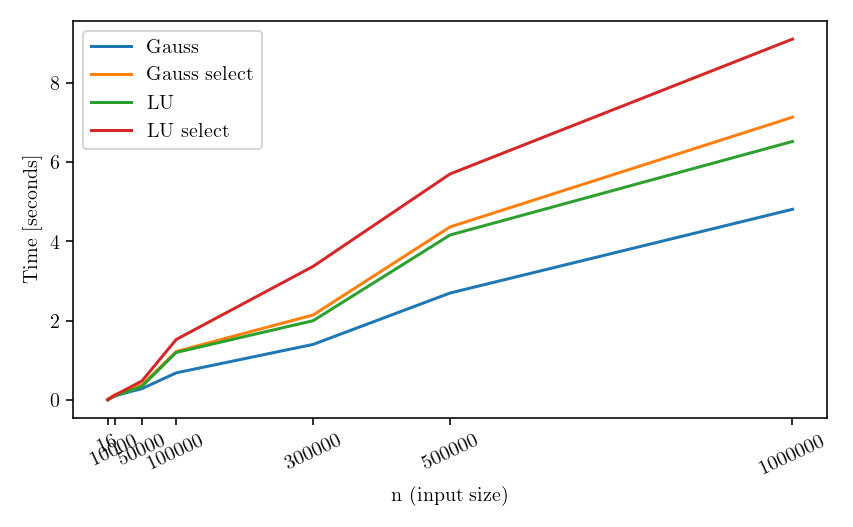
\includegraphics[width=\columnwidth]{runtime.png}
\caption{The running time of each test against the size of the matrix $\bm{M}$.}
\label{fig:runtime}
\end{figure}

The running time of each of the tests is presented in Figure \ref{fig:runtime}.
With minor deviations due to computer load or compilation time, the time grows
linearly with respect to the input size as predicted. Methods which use partial
selection are slightly slower (by a constant factor) compared to their
non-selecting counterparts. Similar solutions using the generic implementation
of a sparse matrix from Julia's standard library achieve considerably worse
results.

\begin{figure}[ht]
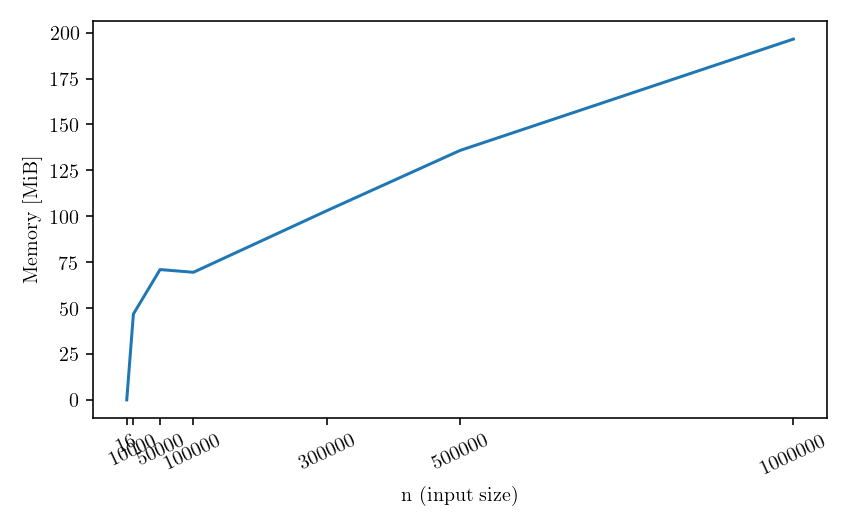
\includegraphics[width=\columnwidth]{memory.png}
\caption{The peak committed memory reported by the Linux \code{time} utility
when running the Gaussian elimination test against the size of the matrix
$\bm{M}$.}
\label{fig:memory}
\end{figure}

The memory usage of the Gaussian elimination test is presented in Figure
\ref{fig:memory}. At small input sizes the committed memory grows rapidly but
linearly. At larger sizes the memory footprint remains linear but this time with
a different, smaller coefficient. The abnormality might be due to the Julia's
allocator overcommitting memory in the case of small allocations as a
performance optimisation. The other methods are not presented in Figure
\ref{fig:memory} as they achieve the same memory complexity with a slightly
different coefficient, for instance the LU method uses 2 matrices unlike the
Gauss method which only requires 1 matrix, thus simply multiplying the required
memory by 2.

\section{Conclusions}
We have achieved a linear time and linear memory solution to the stated problem
far outperforming any standard solution currently available. The solution is
highly specialised for the given specification to attain the best results in
this particular problem.

Although the standard solutions are state of the art, they are not well suited
to all kinds of problems. As shown, it is immensely desirable to adapt the
standard solutions to the peculiarities of the problem.

\end{document}